% This is samplepaper.tex, a sample chapter demonstrating the
% LLNCS macro package for Springer Computer Science proceedings;
% Version 2.20 of 2017/10/04
%
\documentclass[runningheads]{llncs}
%
\usepackage{graphicx}
\usepackage{hyperref}
\usepackage{amsmath}
\usepackage{tabularx}
\usepackage{ragged2e,booktabs,caption}
\usepackage{amsfonts}
\usepackage{amssymb}
\usepackage{listings}
\usepackage{algorithm}
\usepackage{algpseudocode}
% Used for displaying a sample figure. If possible, figure files should
% be included in EPS format.
%
% If you use the hyperref package, please uncomment the following line
% to display URLs in blue roman font according to Springer's eBook style:
% \renewcommand\UrlFont{\color{blue}\rmfamily}
\lstset{
  basicstyle=\ttfamily,
  columns=fullflexible,
  showstringspaces=false,
  commentstyle=\color{gray}\upshape
}

\lstdefinelanguage{XML}
{
  morestring=[b]",
  morestring=[s]{>}{<},
  morecomment=[s]{<?}{?>},
  stringstyle=\color{black},
  identifierstyle=\color{darkblue},
  keywordstyle=\color{cyan},
  morekeywords={xmlns=,version,type,
  Tr}% list your attributes here
}
\begin{document}
%
\title{Mersul Trenurilor\thanks{Project proposed by Continental}}
%
%\titlerunning{Abbreviated paper title}
% If the paper title is too long for the running head, you can set
% an abbreviated paper title here
%
\author{Tudor Ilade}
%
% First names are abbreviated in the running head.
% If there are more than two authors, 'et al.' is used.
%
\institute{Department of Computer Science, "Alexandru Ioan Cuza" University, Iasi
\vspace{0.5mm}
\email{tudor.ilade@yahoo.com}}
%
\maketitle              % typeset the header of the contribution
%
\begin{abstract}
This paper proposes a design of a concurrent client/server project "Mersul Trenurilor". The projects consists on implementing a basic network protocol that contains a server which concurrently handles various type of requests from multiple clients. The communication client-server is implemented using TCP/IP protocol.

\keywords{Mersul Trenurilor  \and Network \and TCP/IP protocol.}
\end{abstract}
%
%
%
\section{Introduction}
I choose this project because building a scalable app for train scheduling it is a difficult task. Many problems can arose during development such as a great architecture for making the code easy to maintain and extend for developers without affecting the performances whilst serving millions of users concurrently. 

In this paper I will propose an application design of "Mersul Trenurilor" project using network communication. The main focus is on building a scalable architecture that can be easily maintained by developers and easy to use by clients.

\section{Technologies}
\subsection{TCP/IP Protocol}
The project uses as client-server communication protocol the TCP/IP. I am interested to implement a reliable, straightforward way to exchange data without having to worry about lost packets or jumbled data. This feature is important because clients cannot only read information from server, but also can modify existing data from a XML file.

When a client sends a request to the server that modifies data, I want to be sure that the data arrives at server is correct and complete and it is updated accordingly. The integrity and accuracy of data is important, otherwise clients who just want to know when next train leaves, might loose the train because of an incorrect update from a previous request. 

Thus, I find TCP/IP protocol the best fit for this project \cite{ref_url1} because is reliable, connection-oriented and full-duplex. The three-way-shake algorithm facilitates the connection between server and client and guarantees data transmission without any loss.

\subsection{Qt XML C++}
The application will perform Read/Write operations from/to an XML file. This operations will be implemented with the help of Qt XML C++ Classes module. \cite{ref_url3}

\subsection{Requirements}

\par The server has been developed with the help of CMake files. The development process has been conducted using Qt Creator. Before running the server, Qt 6.4.1 version should be installed.\cite{qt}

\section{Architecture}

The architecture of application is presented in the following diagram:

\subsection{Server}
\hspace*{-1.2in}
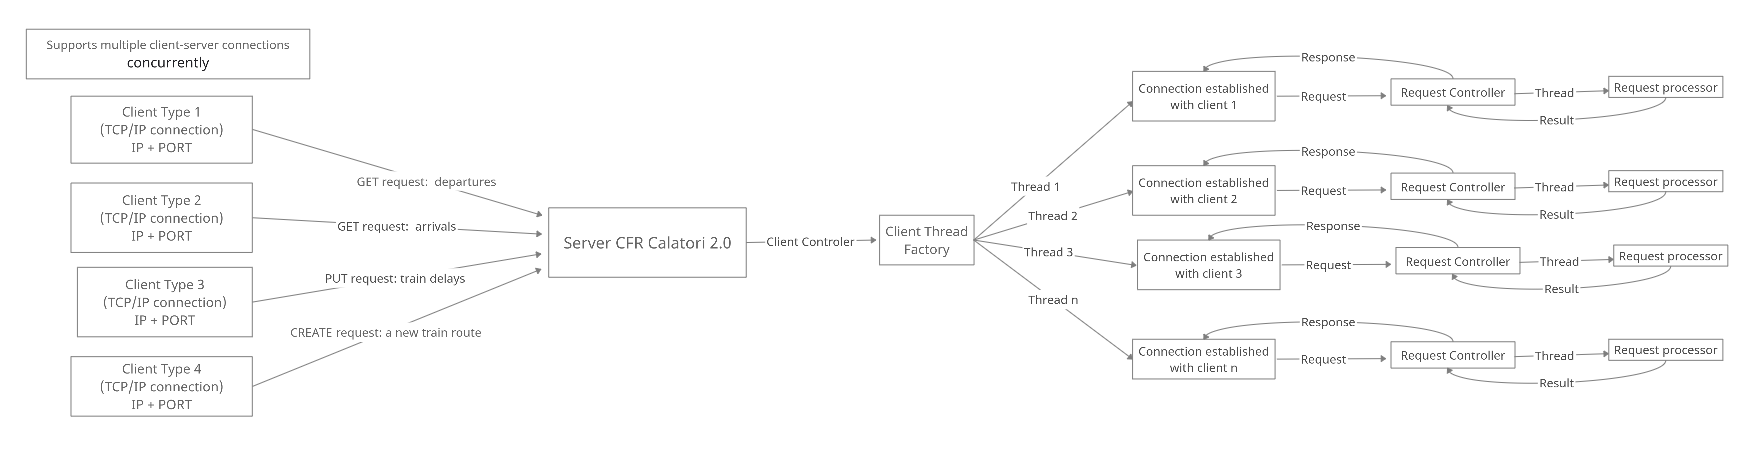
\includegraphics[scale=0.34]{retele.png}


The application will support two classes of commands:

$\rightarrow$ Retrieving data

$\rightarrow$ Manipulating data

Retrieving data commands will consist in GET requests, as follows:

\begin{enumerate}
    \item Client type 1 $\rightarrow$ DEPARTURES: Any connected client can ask for information about departures of trains in the current day.
    \item Client type 2 $\rightarrow$ ARRIVALS: Any connected client can ask for information about arrivals of trains from the following hour or current day.
\end{enumerate}

 For ARRIVALS/DEPARTURES commands, I will implement four flags: 
 \begin{enumerate}
        \item $-stationPS$
        \item $-stationD$
        \item $-fromHour$
        \item $-toHour$
 \end{enumerate}

The format of ARRIVALS/DEPARTURES command is:

\begin{gather*}
   \hspace*{-2cm}\textbf{GET} -stationPS <target> -stationD <dest> -fromHour <HH:MM> -toHour <HH:MM>
\end{gather*}

 \textbf{GET} - type of request. The GET commands are: \textbf{ARRIVALS} for arrivals and \textbf{DEPARTURES} for departures.
 
\textbf{-stationPS} - specifies the target railway station from where trains departs/arrives. This flag is mandatory, which means that the command will not be executed and it sends back appropriate message.

\textbf{-stationD} - specifies the railway station of interest. When it is used in combination with \textbf{-stationPS}, only trains that departs/arrives from target station and head towards station of interest will be displayed. This flag is optional.

\textbf{-fromHour} - specifies the starting hour for displaying arrivals/departures of trains. If it is used, displays trains that arrives/departs in the next hour. (-fromHour + 1h). Default is midnight. If it is not used, will be displayed all the departures/arrivals from that day.

\textbf{-toHour} - specifies the stopping hour for displaying arrivals/departures of trains. If it is used, displays trains that arrives/departs starting from midnight until given hour. If it is used in combination with -fromHour flag, then all trains that arrives/departs in the time frame provided by the 2 flags will be displayed.

\par Example:
\begin{gather*}
   \hspace*{-2cm}\textbf{DEPARTURES}  -stationPS  \; Cluj-Napoca -stationD  \; Huedin -fromHour \; 11:23 -toHour \; 23:30
\end{gather*}

\par Client type 3 $\rightarrow$ UPDATE: Any connected client can modify the schedule details of a train by providing delay time in minutes.

\textbf{UPDATE} command has the following the format:  
\begin{gather*}
   \hspace*{-2cm}\textbf{UPDATE} \;\;-train <id> -delay <minutes> -fromStation <name> -toStation <name>
\end{gather*}

\textbf{-train} - specifies the train ID to which delay time should be added. The train ID is a combination of Type of train and a number (e.g IR322, R3322). The flag is mandatory.

\textbf{-delay} - specifies delay time which should be added to a given train. The delay time has format MM (minutes). The flag is mandatory.

\textbf{-fromStation} - specifies the station from where the delay should be propagated. If it is not specified, the delay will be propagated from first station on the train route. The flag is optional.

\textbf{-toStation} - specifies the station where the propagation of delay time should stop. If it is not specified, the delay will stop at the last station on the train route. The flag is optional.

If \textbf{-fromStation} and \textbf{-toStation} are not specified, the delay time will be adjusted to the entire train route. Any combination these two flags results in an adjustment only between specified stations. If station specified by  \textbf{-toStation} is located before \textbf{-fromStation}, the command will be considered invalid.

\textbf{UPDATE} command is thread safe.

From the \textbf{GET Requests} family, I implemented a \textbf{ROUTE} command which has the main responsability to display the train route.
\textbf{MAN} command has the following the format:  
\begin{gather*}
    \textbf{ROUTE} \;\;-train <train\_id>
\end{gather*}

\textbf{-train} - displays the train route of the train ID supplied.

The server has implemented a manual command which provides information about aforementioned commands and some examples how them should be used.

\textbf{MAN} command has the following the format:  
\begin{gather*}
    \textbf{MAN} \;\;-info <command>
\end{gather*}
Command arguments are: ARRIVALS, DEPARTURES and UPDATE.

Example:

\begin{gather*}
    \textbf{MAN} \;\;-info \; \textbf{UPDATE}
\end{gather*}

The command will display information about update command and how it should be used.

\subsection{Client}
The client architecture is presented bellow:

\vspace{5mm}
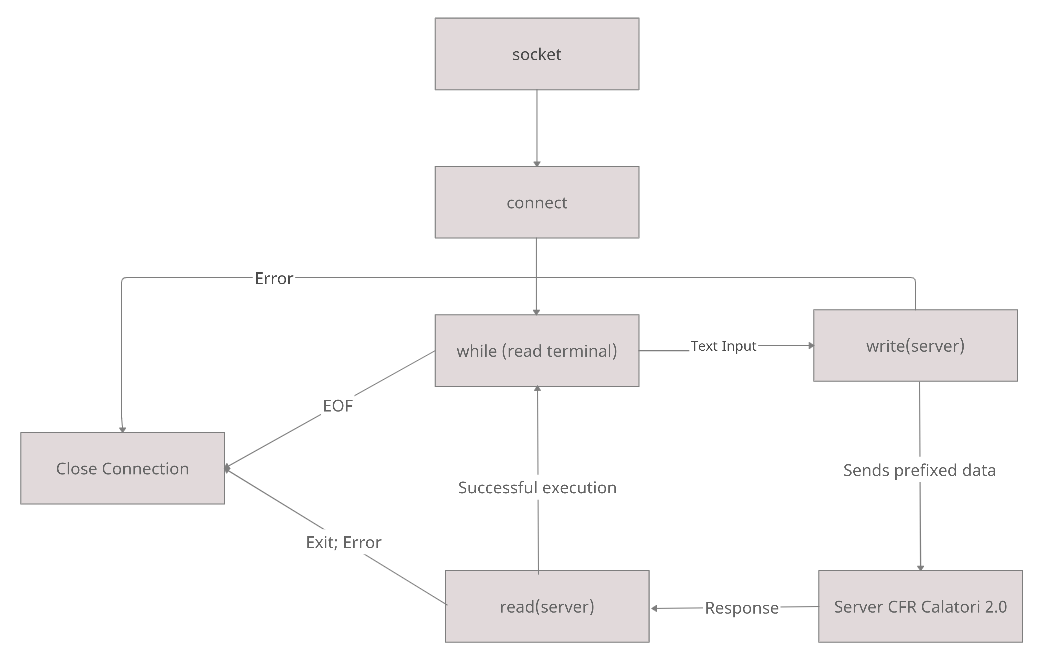
\includegraphics[scale=0.35]{client.png}
\vspace{5mm}

As the main focus is on developing the server, the Client has a simple implementation that consists of three elements:
\begin{enumerate}
    \item Reading data from Terminal until EOF is parsed.
    \item Sends data to server
    \item Read data from server
\end{enumerate}

\section{Implementation}

All clients are served concurrently. The mechanism to serve clients in parallel will be based on multithreading.
This mechanism is implemented with the help of a factory design pattern called Client Thread Factory. Clients are served to Client Thread Factory by a Client Controller.

The Client Controller is a class that has the main responsability of listening and serving new clients, once the connection is successfully established, to Client Thread Factory class.

The Client Thread Factory design pattern is responsible with the handling of new connection requests. The problem with handling multiple connection requests at the same time is tackled with a prethreading protection mechanism that serves requests once at a time and send descriptors to the next empty slot from threading pool. This is achieved with the help of \textbf{Accept} primitive. The server uses mutexes for protecting accept() primitive.

The aforementioned design patterns are implemented as follows:

\vspace{5mm}

\hspace*{-0.3in}
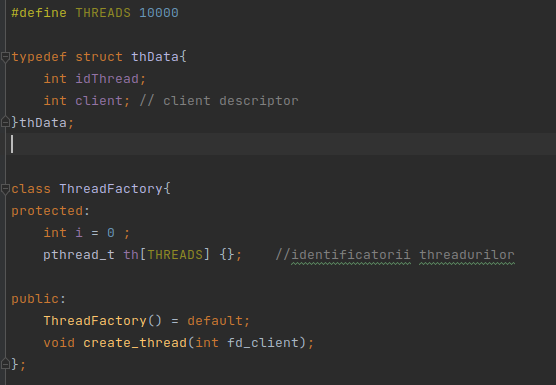
\includegraphics[scale=0.35]{thread_factory.png}
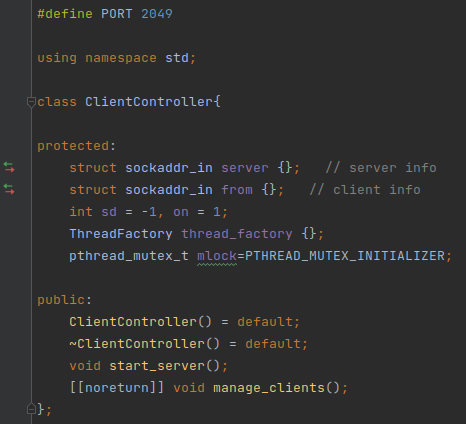
\includegraphics[scale=0.35]{client_Controller.png}

\vspace{5mm}



After client is successfully connected to server, clients can now send requests to server. All the requests are handled by a Request Controller. Its main responsabilities are:


\begin{enumerate}
    \item Receive request
    \item Send the request to Command Factory and convert it to corresponding Command
    \item Handle the Command to Command Manager
    \item Queue the command
\end{enumerate}

Requests are transformed into the corresponding command by CommandFactory class. Commands are implemented with the help of a Command abstract class that is inherited by all available commands. Commands instances store all the relevant info needed for processing, such as client descriptor, CommandResult. Once the request is converted in command by CommandFactory, it is parsed to Command Manager to queue it. 

\vspace{5mm}

\hspace*{-1.3in}
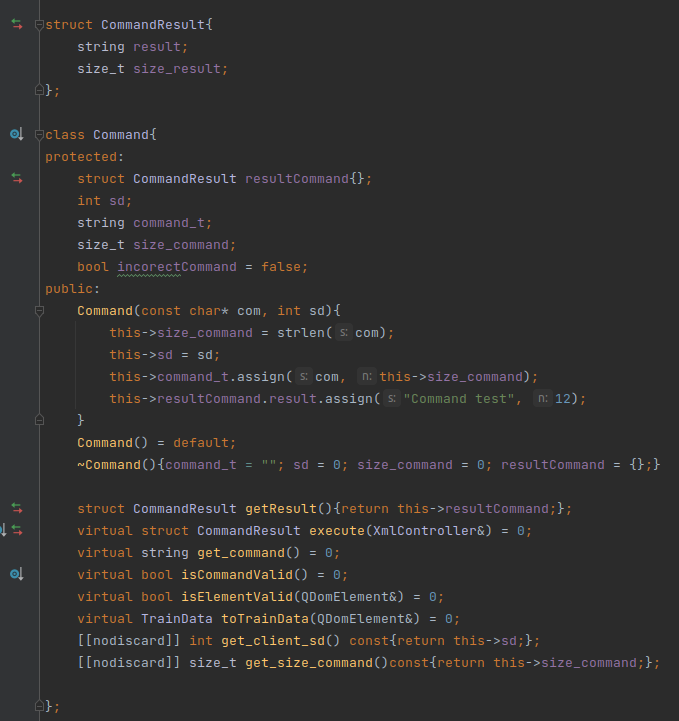
\includegraphics[scale=0.3]{commandABC.png}
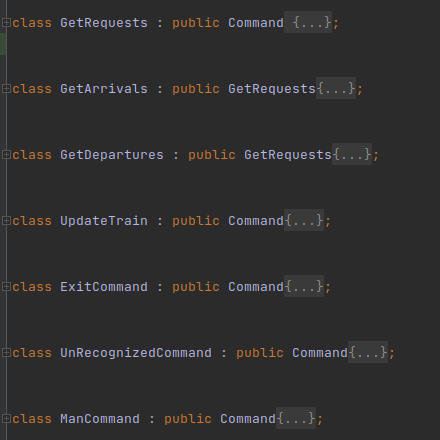
\includegraphics[scale=0.3]{commands.png}
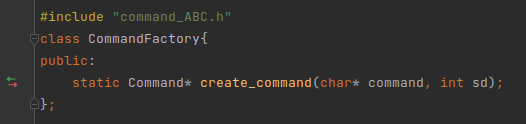
\includegraphics[scale=0.3]{cmd_Factory.png}

The result of \textbf{GET} request is stored with the help of TrainData class. TrainData class stores information about one route which meet the requirements given by command. After processing the entire XML, all eligible routes are stored in a vector of TrainData instances which is converted into a string. The result of this process is then transformed into a CommandResult instance and sent back to client.
\vspace{2mm}

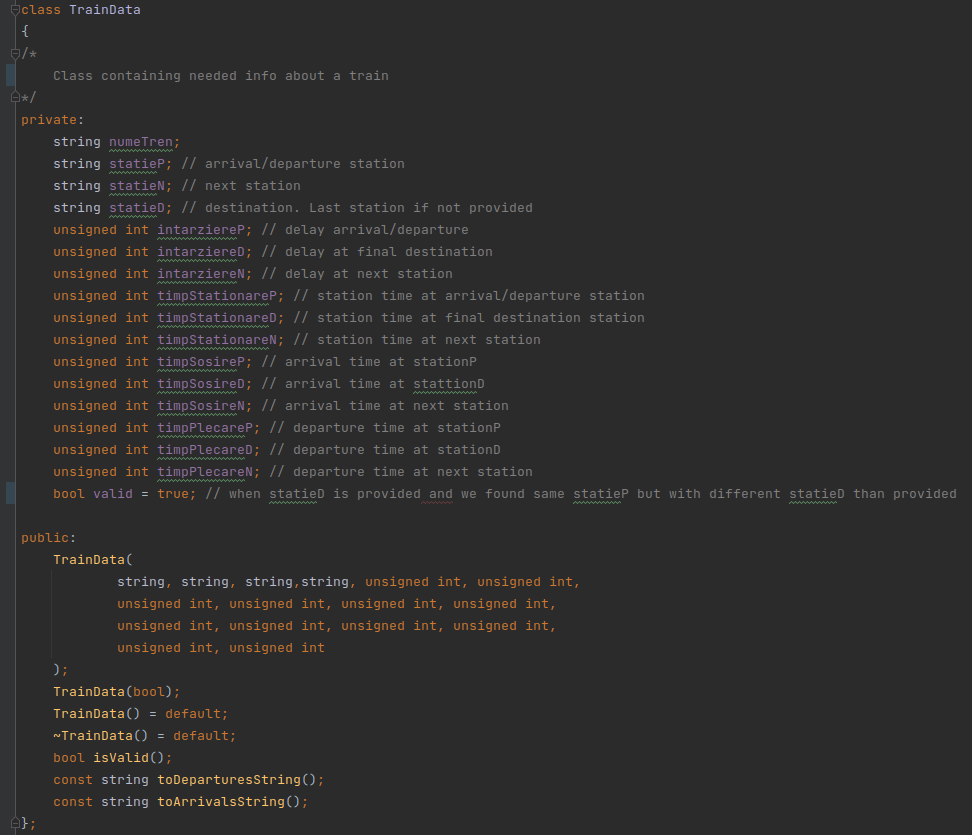
\includegraphics[scale=0.3]{traindata.png}

The Command Manager implements a Command Queue where requests are stored and served according to FIFO rule. The Command Manager has its own threading pool from where it constantly checks the queue. If any command is added to queue, it will be popped from top of the queue and sent to execution. Once the result is obtained, it sends the response to the client. Afterwards the Command Manager will look at Command Queue and send to processing the next command.

\hspace{+1in}
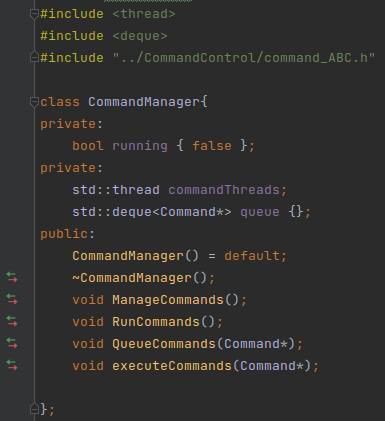
\includegraphics[scale=0.5]{command_manager.png}


The mechanism of reading/writing the XML file is done concurrently. In the implementation, will be used a locks to prevent data race condition\cite{ref_url2} Each client will read the data is available at the time of processing. For update requests pthread\_mutex\_t mutex is used.

The XML File used is a sample that is actually used in production by cfrcalatori \cite{datagov}.It has the following structure:

\begin{lstlisting}
<?xml version='1.0' encoding='UTF-8'?>
<XmlIf encoding="UTF-8" xmlns:xsi="http://www.w3.org/2001/XMLSchema-instance" xsi:noNamespaceSchemaLocation="trnIfSchema_v4.xsd" version="1.0">
 <XmlMts>
  <Mt Versiune="1" DataExport="20151228" MtValabilDeLa="20151213" MtValabilPinaLa="20161210">
   <Trenuri>
    <Tren KmCum="57100.0" Numar="2872" Operator="6100826" Putere="E" CategorieTren="R" Lungime="250" Servicii="2" Rang="4" Tonaj="500" Proprietar="6100826">
     <Trase>
      <Trasa Tip="Implicita" Id="1" CodStatieInitiala="23428" CodStatieFinala="10938">
       <ElementTrasa Secventa="1" DenStaOrigine="Târgu Jiu" OraP="44400" 
       Ajustari="0" Restrictie="0" DenStaDestinatie="Ram. Budieni" 
       VitezaLivret="80" StationareSecunde="0" Rco="R" Km="1600" 
       Lungime="250" TipOprire="N" CodStaDest="27888" Tonaj="500" 
       OraS="44580" Rci="R" CodStaOrigine="23428"/>
       <ElementTrasa Secventa="3" DenStaOrigine="Amaradia" OraP="45000"
       Ajustari="0" Restrictie="0" DenStaDestinatie="Drăguţeşti h."
       VitezaLivret="80" StationareSecunde="60" Rco="R" Km="3400"
       Lungime="250" TipOprire="C" CodStaDest="24587" Tonaj="500"
       OraS="45300" Rci="R" CodStaOrigine="24575"/>
       <ElementTrasa Secventa="4" DenStaOrigine="Drăguţeşti h."
       OraP="45360" Ajustari="0" Restrictie="0"
       DenStaDestinatie="Cârbeşti Hm." VitezaLivret="80"
       StationareSecunde="60" Rco="R" Km="3000" Lungime="250"
       TipOprire="C" CodStaDest="24599" Tonaj="500" OraS="45600"
       Rci="R" CodStaOrigine="24587"/>
       <ModificariInParcurs/>
      </Trasa>
     </Trase>
     <Grupe/>
     <RestrictiiTren>
      <CalendarTren DeLa="20151213" Tip="Da" Id="1" Zile="16767" PinaLa="20161210"/>
     </RestrictiiTren>
    </Tren>
   </Trenuri>
  </Mt>
 </XmlMts>
</XmlIf>
\end{lstlisting}

The entire I/O operations of the XML are done with the help of XmlController class. The constructor of XmlController opens the XML and loads it to buffer on which the operations are performed. Before any command is executed, the XML buffer is refreshed to load the latest data, in case any update has been made.

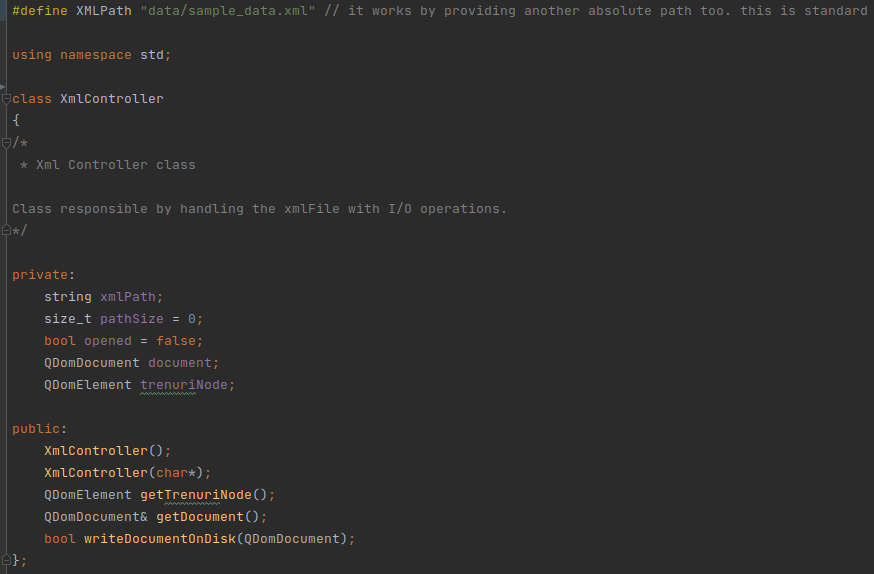
\includegraphics[scale=0.3]{xmlcontroller.png}



The communication between client and server are in both way prefixed with the length of data ready to be sent. The prefixed communication consists in writing the size of data as integer at the beginning of each message, followed by data.

\subsubsection{Scenario}


I will present some scenarios how the application should be used and how it behaves when certains commands are sent. Let us suppose client sends an invalid request, meaning a command that is not recognized by server. In this case, server will receive the request and will convert it in an UnRecognizedCommand. After the command is queued, it starts execution and sends back to client an appropiate message.

In case client wants to close connection, has to send an exit request that will be processed by server. The server shuts down the connection with client once executes all commands from queue and sends all responses to client. Once EXIT response is received from server, the connection is shutted down. In case if a connection is closed abnormal (i.e. SIGINT, SIGTSTP or SIGTERM), a handler is attached to these signals which ensures that the connection will be shut down correctly on the server side.

Another edge case is when the server crash for some reason and is closed unexpectedly. In this scenario, all the connections with all clients are closed and all threads are joined.

Let us suppose the user sends a command where he or she duplicates the the flags and arguments. For example, consider the following command:

\begin{gather*}
   \hspace*{-2cm}\textbf{DEPARTURES}  -stationPS  \; Cluj Napoca -stationPS  \; Huedin
\end{gather*}

In this case, the command will be considered valid. The behavior is that the server consider only the last argument from the chain of arguments when they are the same. Here, only departures from Huedin will be displayed, and not Cluj Napoca. If a flag is invalid, the command will be considered invalid, even though the other ones are valid.



\section{Conclusion}
This is my proposed implementation of the Mersul Trenurilor project. Further improvements can be done by adding more features to it. Some possible features that can be added are:

$\rightarrow$ The possibility of client to choose the type of connection they want (TCP/IP or UDP) for GET requests. In this case, usually the client wants to know fast some details about a train. In majority of cases this protocol will yield the desired result without data loss. And even so, the Client can send another request if he or she sees that nothing has been returned. The majority of requests of this server will be of type GET, rather than PUT or CREATE. Thus, the feature can result into much faster exchange of information.

$\rightarrow$ A backup mechanism implemented for XML file to make sure that in case of failures, data is backed up periodically and prevents massive data loss.

$\rightarrow$ A secured connection by providing a TOKEN in case of writing data on XML. The TOKEN can be generated uniquely in UUID4 format, thus only trusted users can perform Write operations.


\begin{thebibliography}{8}

\bibitem{ref_book1}
W. Richard Stevens, Bill Fenner, Andrew M. Rudoff,
UNIX Network Programming Volume 1, Third Edition: The Sockets Networking API, 3rd. ed. Publisher,
Addison Wesley (2003)
\bibitem{ref_url1}
Computer Networks Homepage, \url{https://profs.info.uaic.ro/~computernetworks/index.php}. Last access 1 dec 2022
\bibitem{ref_url2} Mutex lock for threads, \url{https://www.geeksforgeeks.org/mutex-lock-for-linux-thread-synchronization/}. Last access 1 dec 2022

\bibitem {datagov} XML sample from government of Romania \url{https://data.gov.ro/dataset/c4f71dbb-de39-49b2-b697-5b60a5f299a2/resource/d0ec6682-5c00-4666-89dc-6a5e7831b8dd/download/mers-trensntfc2015-2016.xml}. Last access 25 dec 2022
\bibitem{ref_url3}
Qt XML docpage, \url{https://doc.qt.io/qt-6/qtxml-module.html}. Last access 26 dec 2022
\bibitem{qt}
Qt downloader - \url{https://www.qt.io/download}. Last access 26 dec 2022
\end{thebibliography}
\end{document}
